\addtocounter{chapter}{-1}
\chapter{Advice for reading this book}
\section{Prerequisites}
The main prerequisite is some amount of mathematical maturity:
the ability to read/write proofs, and follow mathematical arguments, etc.

I also assume the reader is familiar with foundational notions such
as sets and functions (e.g.\ ``what is a bijection?'').
If not, one should consult \Cref{ch:sets_functions}.

\section{Graph of chapter dependencies}
There is no need to read this book in linear order.
Here is a plot of where the various chapters are relative to each other.
In my opinion, the really cool stuff is the later chapters,
which have been bolded below.
Dependencies are indicated by arrows;
dotted lines are optional dependencies.
I suggest that you simply pick a chapter you find interesting,
and then find the shortest path.
With that in mind, I hope the length of the entire PDF is not intimidating.

Many of the later parts are subdivided into ``Part I'' and ``Part II''.
In general, the second part is substantially harder than the first part.
If you intend to read a large portion of the text,
one possible thing to do is to read all the Part I's
before reading all the Part II's.

I have tried to keep the chapters short, and no more than 15 pages each.
Several hints and solutions can be found in \Cref{app:hints,app:sol}.
\todo{rewrite}
%The original intention was that each chapter could be digested
%(albeit with some effort) in a couple of hours,
%true to the subtitle of ``bedtime stories''.
%Unfortunately, I think in many of the Part II's this is no longer true.

%The oddball in this graph is the category theory.
%Basically, the more examples from other chapters you know,
%the easier this chapter will be to digest.
%But \emph{strictly} speaking, you don't need any prerequisites at all;
%the subject is very ``combinatorial''.

%\chapter*{Graph of Chapter Dependencies}
%\addcontentsline{toc}{chapter}{Graph of Chapter Dependencies}

\bgroup
\renewcommand{\href}[1]{} % temp disable links
\renewcommand{\solidwidth}{0.7pt}
\renewcommand{\boldwidth}{1.5pt}

\setcounter{diagheight}{50}
\begin{chart}
\halfcourse 10,45:{Chapters 1,3}{Groups}{}
\halfcourse 48,45:{Chapter 2}{Spaces}{}
\halfcourse 48,35:{Chapters 4-5}{Topology}{}
\halfcourse 63,45:{Chapter 6}{Modules}{}
\halfcourse 63,35:{Chapters 7-9}{Lin Alg}{}
\halfcourse 5,35:{Chapter 10}{Grp Actions}{}
\halfcourse 5,20:{Chapter 11}{Grp Classif}{}
\halfcourse 30,35:{Chapter 12-13}{Ideals}{}
\reqhalfcourse 55,10:{Chapters 14-16}{Cmplx Ana}{}
\halfcourse 58,19:{Chapters 17-19}{Quantum}{}
\reqhalfcourse 30,10:{Chapters 20-22}{Alg Top 1}{}
\reqhalfcourse 30,22:{Chapters 23-25}{Cat Th}{}
\halfcourse 65,25:{Chapters 26-29}{Diff Geo}{}
\reqhalfcourse 20,0:{Chapters 30-35}{Alg Top 2}{}
\reqhalfcourse 42,10:{Chapters 36-40}{Alg NT 1}{}
\reqhalfcourse 42,0:{Chapter 41-45}{Alg NT 2}{}
\reqhalfcourse 35,45:{Chapters 46-49}{Rep Theory}{}
\reqhalfcourse 16,10:{Chapters 50-53}{Alg Geom 1}{}
\halfcourse 6,0:{Chapters 54-56}{Alg Geom 2}{}
\reqhalfcourse 65,0:{Chapters 57-63}{Set Theory}{}

\prereqc 30,35,35,45;0:   % Ideals -> Rep Th
\prereqc 63,35,35,45;0:   % Lin Alg -> Rep Th
\coreqc  30,22,35,45;50: % Cats -> Rep Th
\prereqc 63,35,58,19;30:  % Lin Alg -> Quantum
\prereqc 48,45,65,25;-20: % Spaces -> Diff Geo

\prereqc 10,45,30,22;0:   % Gp -> Cat Th
\coreqc  30,35,30,22;0:   % Ideals -> Cat Th
\coreqc  48,45,30,22;0:   % Space -> Cat Th
\coreqc  63,35,30,22;10:  % Lin Alg -> Cat Th
\prereqc 63,35,65,25;0:   % Lin Alg -> Diff Geo
\coreqc  48,35,30,22;-10: % Top -> Cat Th
\coreqc  30,22,16,10;0:   % Cat Th -> AG2
\prereqc 63,45,30,35;0:   % Module -> Ideal

\prereqc 30,10,20,0;0:    % AT1 -> AT2
\prereqc 30,22,20,0;20:   % Cat -> AT2
\coreqc  30,22,30,10;0:   % Cat -> AT1

\prereqc 10,45,5,35;0:    % Grp -> Grp Act
\prereq   5,35,5,20:      % Grp Act -> Grp Class
\prereq  48,45,48,35:     % Space -> Top
\prereqc 48,35,30,10;0:   % Top -> AT1
\prereqc  5,35,30,10;0:   % Grp Act -> AT1
\prereqc 48,35,55,10;-30: % Top -> Cmplx Ana
\coreqc  10,45,30,35;0:   % Grp -> Ideals
\prereqc 30,35,42,10;0:   % Ideals -> ANT1
\prereq  63,45,63,35:     % Modules -> Linalg
\prereq  63,45,42,10:     % Modules -> ANT1
\coreqc  63,35,42,10;0:   % Lin Alg -> ANT1
\prereqc 30,35,16,10;0:   % Ideals -> AG1
\prereqc 48,35,16,10;-30: % Top -> AG1
\prereqc 42,10,42,0;0:    % ANT1 -> ANT2
\prereqc 16,10,6,0;0:     % AG1 -> AG2
\prereqc 30,22,6,0;80:     % Cat -> AG2
\prereqc  5,35,42,0;-30:  % Grp Act -> ANT2
\end{chart}
\egroup


\eject

\section{Questions, exercises, and problems}
In this book, there are three hierarchies:
\begin{itemize}
	\ii A \emph{question} is intended to be offensively easy,
	mostly a chance to help you internalize definitions.
	If you find yourself unable to answer one or two of them,
	it probably means I explained it badly and you should complain to me.
	But if you can't answer many,
	you likely missed something important: read back.
	\ii An \emph{exercise} is marginally harder.
	The difficulty is like something you might see on a high-school math contest.
	Often I leave proofs of theorems and propositions as exercises
	if they are instructive and at least somewhat interesting.
	\ii Each chapter features several \emph{problems} at the end.
	Some of these are easy, while others are
	legitimately difficult olympiad-style problems.
	There are three types:
	\begin{itemize}
		\ii \textbf{Normal problems},
		which are hopefully fun but non-central.
		\ii \textbf{Daggered problems},
		which are (usually interesting) results that one should know,
		but won't be used directly later.
		\ii \textbf{Starred problems},
		which are results which will be used later on.\footnote{%
			A big nuisance in college for me was that,
			every so often, the professor
			would invoke some nontrivial result from the homework:
			``we are done by PSet 4, Problem 8'',
			as if I remembered what that was.
			I wish they could have told me in advance
			``please take note of this, we'll use it later on''.
		}
	\end{itemize}
\end{itemize}
Several hints and solutions can be found in \Cref{app:hints,app:sol}.

\gim
Harder problems are marked with \chili's, like this paragraph.
For problems that have three chili's you should probably read the hint.

\begin{center}
	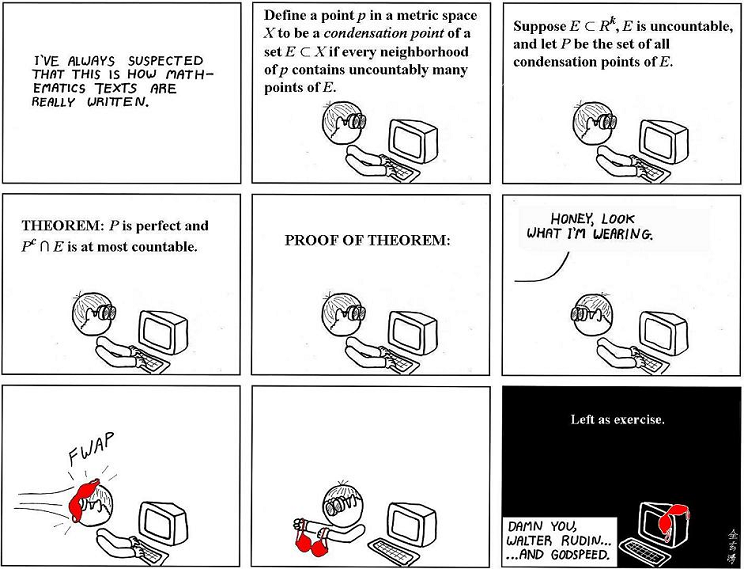
\includegraphics[width=14cm]{media/abstruse-goose-exercise.png}
	\\ \scriptsize Image from \cite{img:exercise}
\end{center}

% I personally find most exercises to not be that interesting, and I've tried to keep boring ones to a minimum.
% Regardless, I've tried hard to pick problems that are fun to think about and, when possible, to give them
% the kind of flavor you might find on the IMO or Putnam (even when the underlying background is different).

\section{Paper}
At the risk of being blunt,
\begin{moral}
Read this book with pencil and paper.
\end{moral}
Here's why:

\begin{center}
	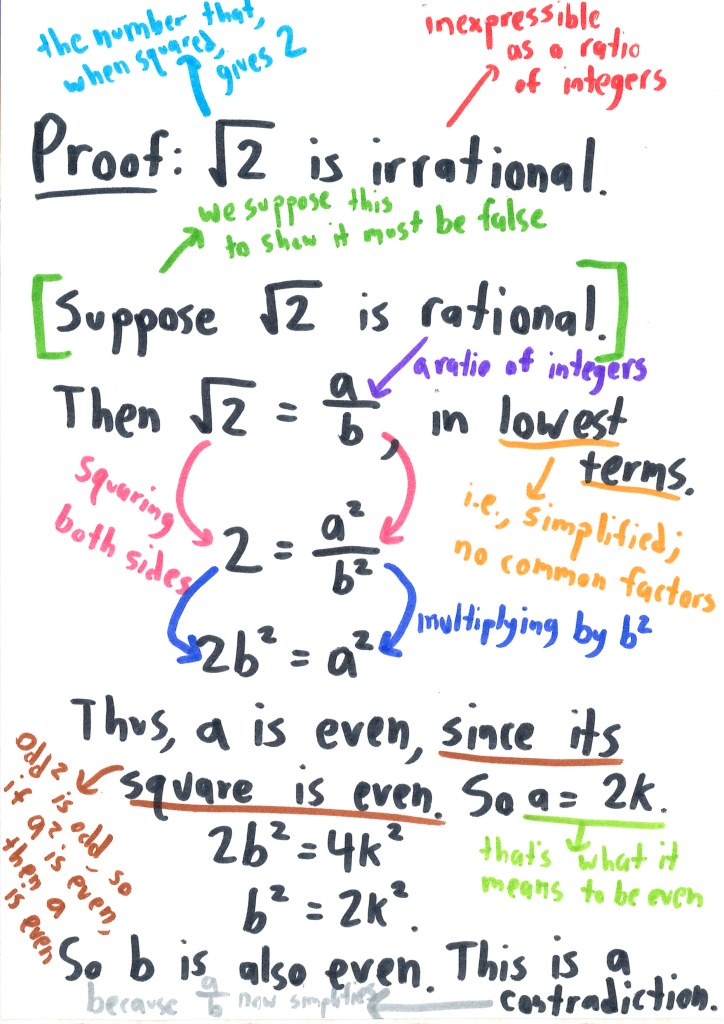
\includegraphics[width=0.5\textwidth]{media/read-with-pencil.jpg}
	\\ \scriptsize Image from \cite{img:read_with_pencil}
\end{center}
You are not God.
You cannot keep everything in your head.\footnote{
	See also \url{https://usamo.wordpress.com/2015/03/14/writing/}
	and the source above.}
If you've printed out a hard copy, then write in the margins.
If you're trying to save paper,
grab a notebook or something along with the ride.
Somehow, some way, make sure you can write. Thanks.

\section{Examples}
I am pathologically obsessed with examples.
In this book, I place all examples in large boxes to draw emphasis to them,
which leads to some pages of the book simply consisting of sequences of boxes
one after another. I hope the reader doesn't mind.

I also often highlight a ``prototypical example'' for some sections,
and reserve the color red for such a note.
The philosophy is that any time the reader sees a definition
or a theorem about such an object, they should test it
against the prototypical example.
If the example is a good prototype, it should be immediately clear
why this definition is intuitive, or why the theorem should be true,
or why the theorem is interesting, et cetera.

Let me tell you a secret.  Whenever I wrote a definition or a theorem in this book,
I would have to recall the exact statement from my (quite poor) memory.
So instead I often consider the prototypical example,
and then only after that do I remember what the definition or the theorem is.
Incidentally, this is also how I learned all the definitions in the first place.
I hope you'll find it useful as well.

\section{Topic choices}
The appendix contains a list of resources I like,
and explanations of pedagogical choices that I made for each chapter.
I encourage you to check it out.

In particular, this is where you should go for further reading!
There are some topics that should be covered in the Napkin,
but are not, due to my own ignorance or laziness.
The references provided in this appendix should hopefully help partially
atone for my omissions.

\section{Conventions and notations}
This part describes some of the less familiar notations and definitions
and settles for once and for all some annoying issues (``is zero a natural number?'').
Most of these are ``remarks for experts'':
if something doesn't make sense, you probably don't have to worry about it for now.

A full glossary of notation used can be found in the appendix.

\subsection*{Sets and equivalence relations}
This is brief, intended as a reminder for experts.
Consult \Cref{ch:sets_functions} for full details.

An \vocab{equivalence relation} on a set $X$ is a relation $\sim$
which is symmetric, reflexive, and transitive.
An equivalence relation partitions $X$ into several \vocab{equivalence classes}.
We will denote this by $X / {\sim}$.
An element of such an equivalence class is a \vocab{representative} of that equivalence class.

I always use $\cong$ for an ``isomorphism''-style relation
(formally: a relation which is an isomorphism in a reasonable category).
The only time $\simeq$ is used in the Napkin is for homotopic paths.

I generally use $\subseteq$ and $\subsetneq$ since these are non-ambiguous,
unlike $\subset$.  I only use $\subset$ on rare occasions in which equality
obviously does not hold yet pointing it out would be distracting.
For example, I write $\QQ \subset \RR$
since ``$\QQ \subsetneq \RR$'' is distracting.

I prefer $S \setminus T$ to $S - T$.

\subsection*{Functions}
Same comments about \Cref{ch:sets_functions} apply as previous section.

Let $X \taking f Y$ be a function.

\begin{itemize}
\ii By $f\pre(T)$ I mean the \vocab{pre-image}
\[ f\pre(T) \defeq \left\{ x \in X \mid f(x) \in T \right\} \]
in contrast to the usual $f\inv(T)$; I only use $f\inv$ for an inverse \emph{function}.

By abuse of notation, we may abbreviate $f\pre(\{y\})$ to $f\pre(y)$.
We call $f\pre(y)$ a \vocab{fiber}.

\ii By $f``(S)$ I mean the \vocab{image}
\[ f``(S) \defeq \left\{ f(x) \mid x \in S \right\}. \]
The notation {``} is from set theory, and is meant to indicate ``point-wise''.
Most authors use $f(S)$, but this is abuse of notation,
and I prefer $f``(S)$ for emphasis.
\textbf{This image notation is probably the least standard in the whole Napkin}.

\ii If $S \subseteq X$, then the \vocab{restriction} of $f$ to $S$
is denoted $f \restrict{S}$,
i.e.\ it is the function $f \restrict{S} : S \to Y$.

\ii Sometimes functions $f : X \to Y$ are \emph{injective} or \emph{surjective};
I may emphasize this sometimes by writing $f : X \injto Y$ or $f : X \surjto Y$, respectively.
\end{itemize}

\subsection*{Rings}
All rings have a multiplicative identity $1$ unless otherwise specified.
We allow $0=1$ in general rings but not in integral domains.

\textbf{All rings are commutative unless otherwise specified.}
There is an elaborate scheme for naming rings which are not commutative,
used only in the chapter on cohomology rings:

\begin{center}
	\small
	\begin{tabular}[h]{|c|cc|}
		\hline
		& Graded & Not Graded \\ \hline
		$1$ not required & graded pseudo-ring & pseudo-ring \\
		Anticommutative, $1$ not required & anticommutative pseudo-ring & N/A \\
		Has $1$ & graded ring & N/A \\
		Anticommutative with $1$ & anticommutative ring & N/A \\ 
		Commutative with $1$ & commutative graded ring & ring \\ \hline
	\end{tabular}
\end{center}

On the other hand, an \emph{algebra} always has $1$,
but it need not be commutative.

\subsection*{Natural numbers are nonzero}
The set $\NN$ is the set of \emph{positive} integers, not including $0$.
In the set theory chapters, we use $\omega = \{0, 1, \dots\}$
instead, for consistency with the rest of the book.

\subsection*{Choice}
We accept the Axiom of Choice, and use it freely.

\section{Further reading}
Recommendations for other reading can be found in \Cref{ch:refs}.
